\section{Motivation}

\begin{frame}{Disclaimer!}
    \[
        \text{Vertex} \iff \text{Point} \iff \text{Vector}
    \]
\end{frame}

\subsection{Similarity Search and \(k\)-NNS}

\begin{frame}{Similarity Search}
    \begin{itemize}
        \item Finding similar \textit{objects}
        \item In CS: Recommendation systems, Information retrieval, Search engine
    \end{itemize}
\end{frame}

\begin{frame}{Similarity Search (in Recommendation System)}
    \begin{figure}[ht]
        \centering
        \hfill
        \begin{subfigure}{0.33\textwidth}
            \centering
            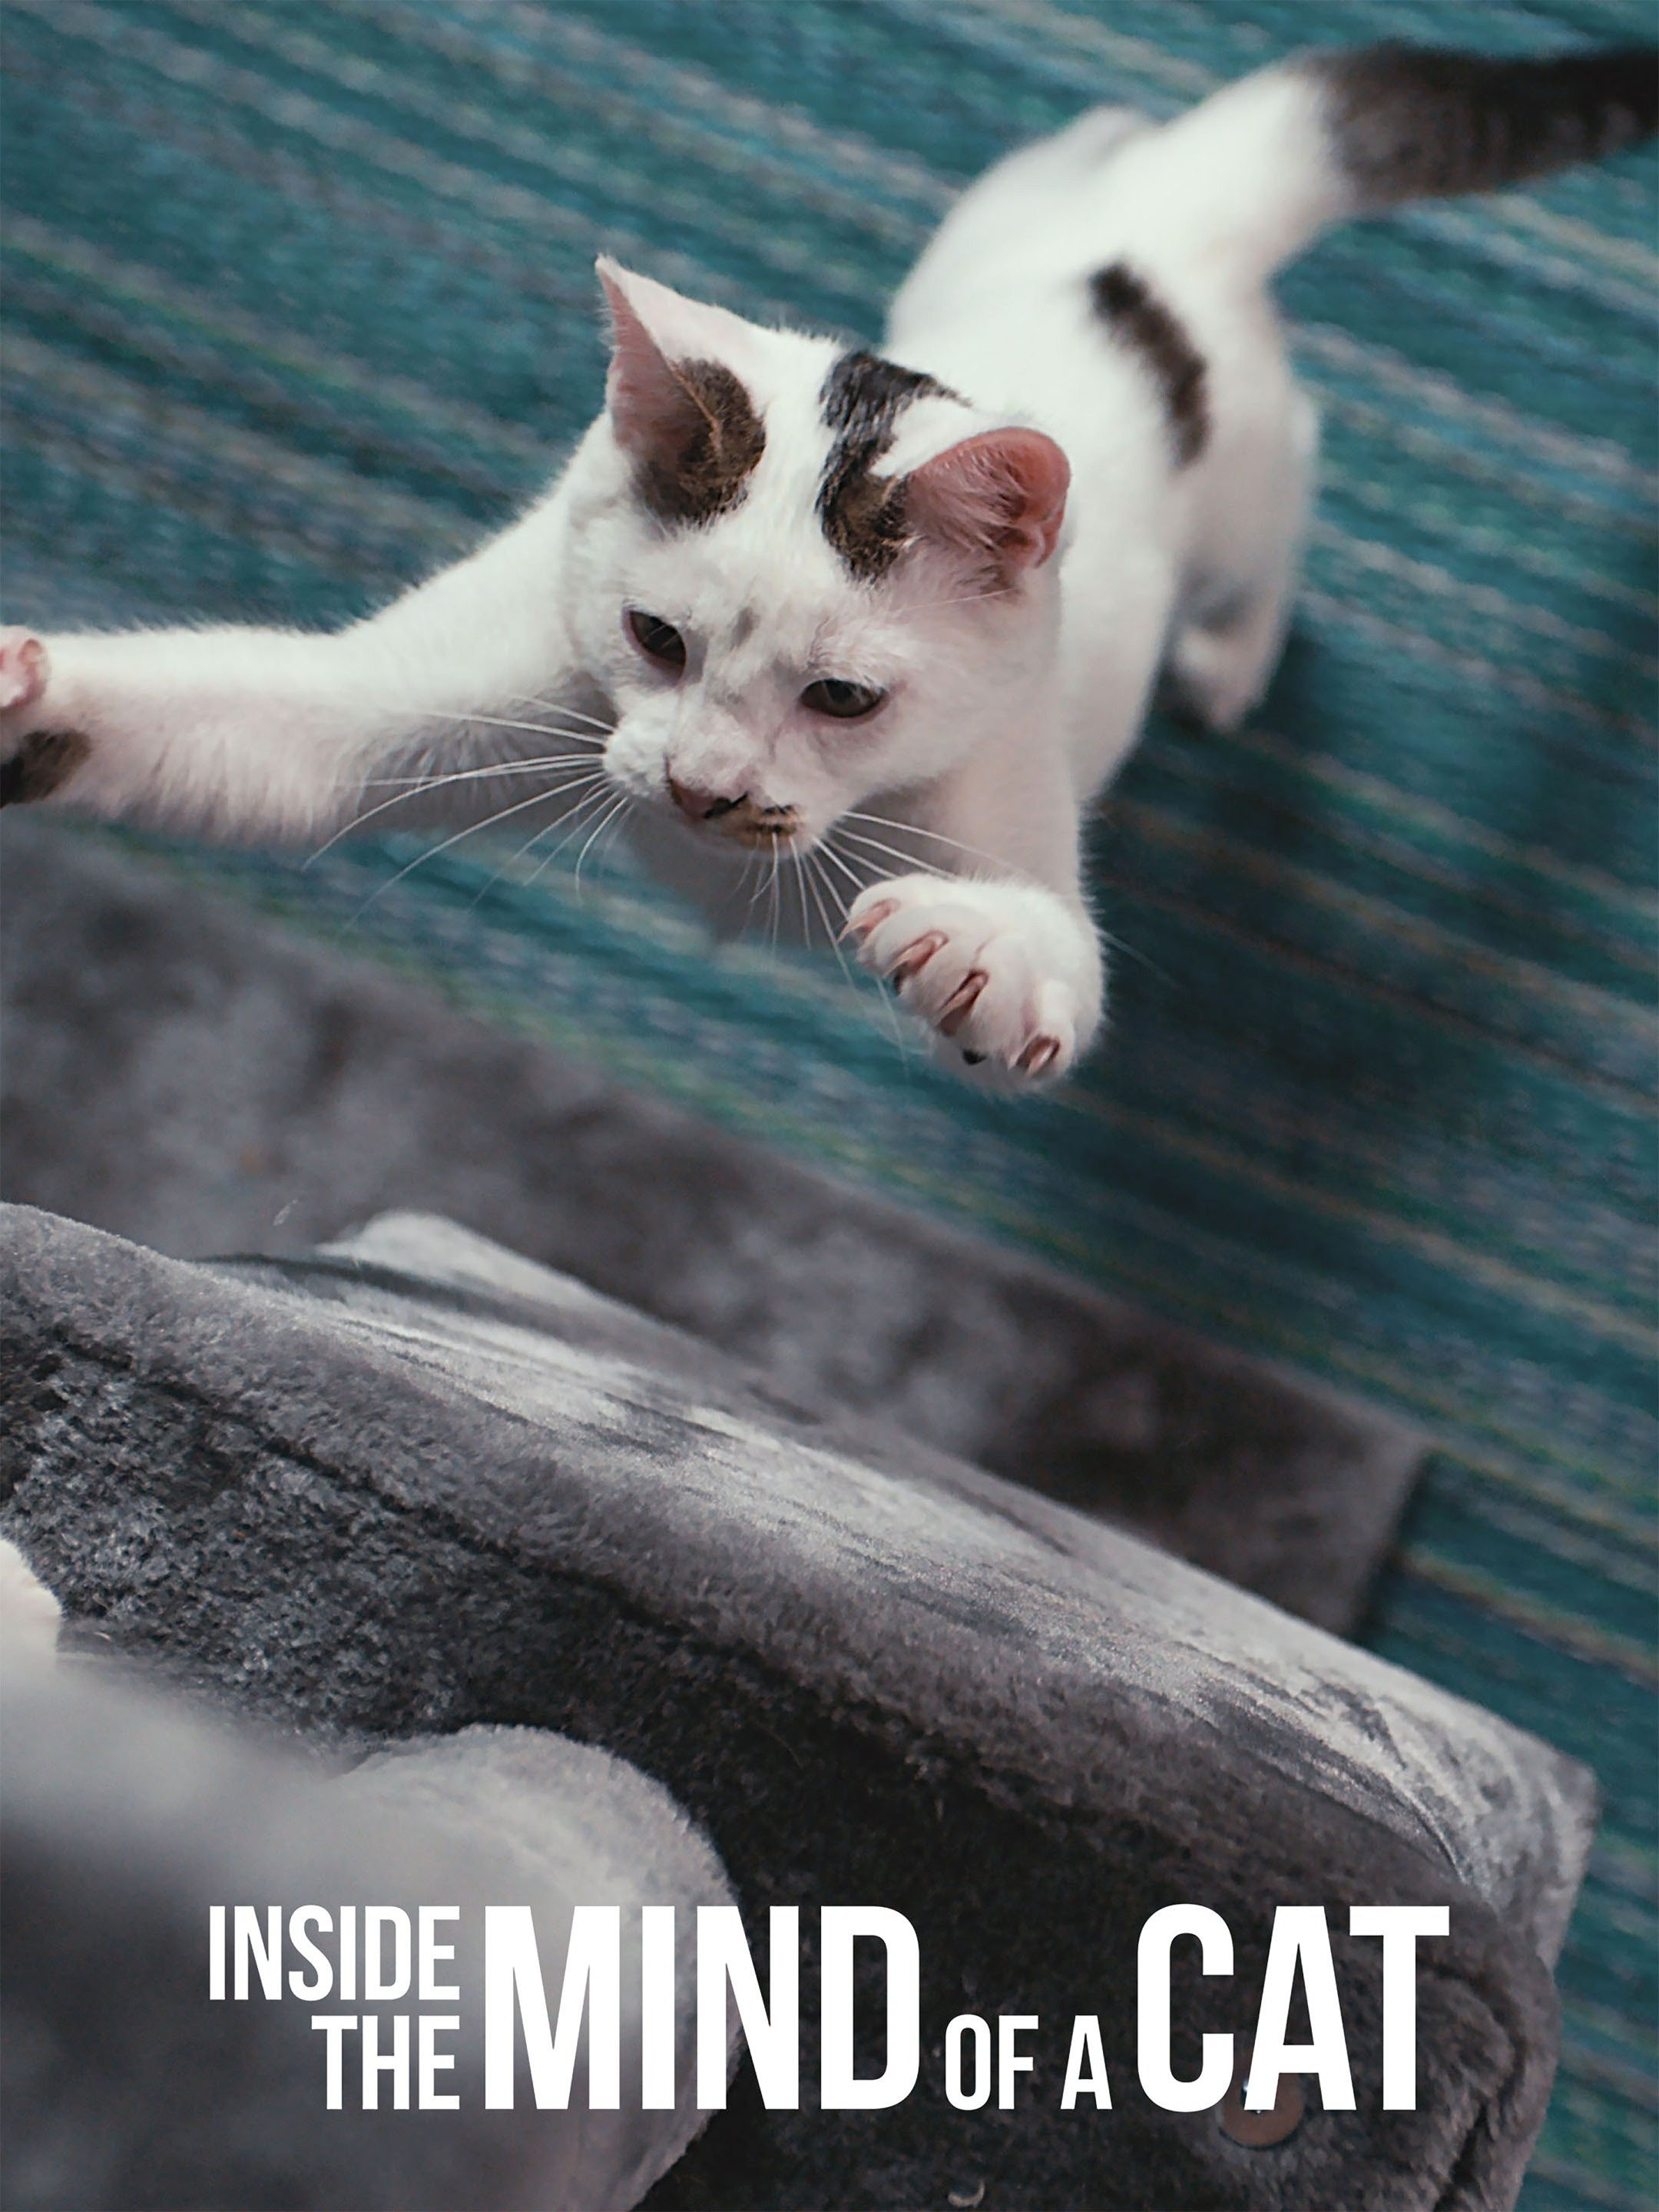
\includegraphics[height=0.69\textheight]{images/inside-the-mind-of-a-cat.jpg}

            {Just watched and loved}
        \end{subfigure}
        \hfill
        \begin{subfigure}{0.27\textwidth}
            \centering
            
\includegraphics[height=0.6\textheight]{images/cat-people.jpg}

            {Choice A}
        \end{subfigure}
        \begin{subfigure}{0.27\textwidth}
            \centering
            
\includegraphics[height=0.6\textheight]{images/jujutsu-kaisen.jpg}

            {Choice B}
        \end{subfigure}
        \hfill
    \end{figure}
\end{frame}

\begin{frame}{Similarity Search (in Math) --- \(k\)-Nearest Neighbor Search}
    \begin{figure}[ht]
        \centering
        \caption*{\textbf{Trade offer}}
        \hfill
        \begin{subfigure}{0.42\textwidth}
            \caption*{You receive}
            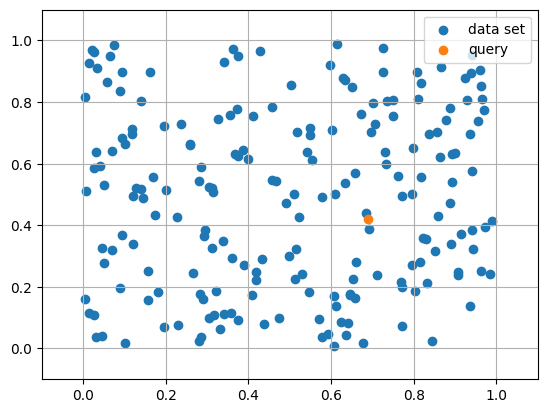
\includegraphics[width=\textwidth]{images/sim-search-init.png}
        \end{subfigure}
        \hfill
        \begin{subfigure}{0.42\textwidth}
            \caption*{I receive}
            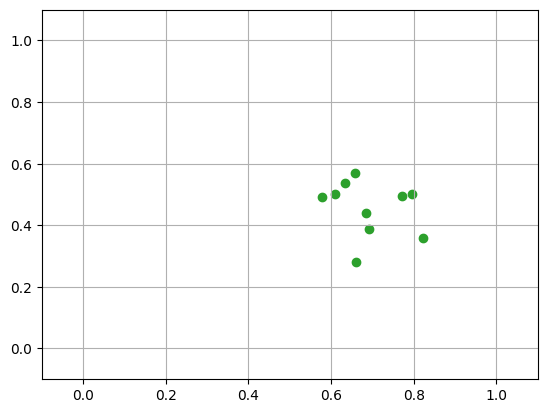
\includegraphics[width=\textwidth]{images/sim-search-knn.png}
        \end{subfigure}
        \hfill
    \end{figure}
\end{frame}

\begin{frame}{Similarity Search (in Math) --- \(k\)-Nearest Neighbor Search}
    \begin{figure}[ht]
        \centering
        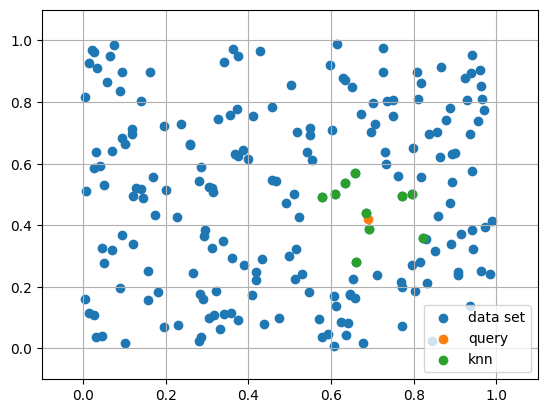
\includegraphics[width=0.5\textwidth]{images/sim-search-final.png}
    \end{figure}
\end{frame}

\begin{frame}{\(k\)-Nearest Neighbor Search}
\begin{definition}[\(k\)-Nearest Neighbor Search]
    Given point set \(\mathcal{P} \subset \mathbb{R}^d\), query point \(q \in \mathbb{R}^d\), and a distance function \(\delta\), we want to find a set \(\mathcal{K} \subseteq \mathcal{P}\) such that \(|\mathcal{K}| = k\) and
    \[
        \max_{p \in \mathcal{K}} \delta(p, q) \leq \min_{p \in \mathcal{P} \setminus \mathcal{K}} \delta(p, q)
    \]
    \end{definition}

    \hfill
    \begin{figure}[ht]
        \centering
        \begin{subfigure}{0.24\textwidth}
            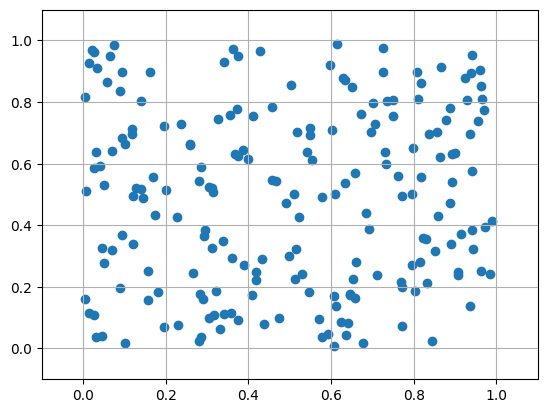
\includegraphics[width=\textwidth]{images/sim-search-P}
            \caption*{\(\mathcal{P}\)}
        \end{subfigure}
    \hfill
        \begin{subfigure}{0.24\textwidth}
            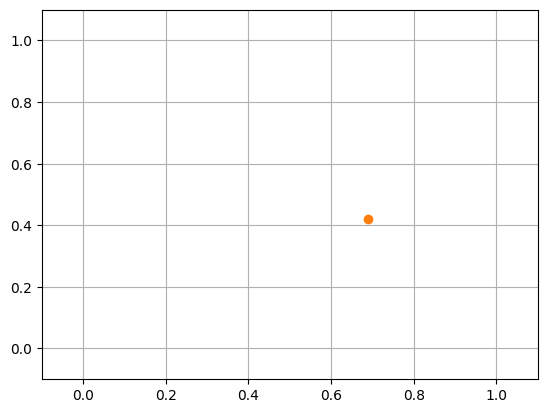
\includegraphics[width=\textwidth]{images/sim-search-q}
            \caption*{\(q\)}
        \end{subfigure}
    \hfill
        \begin{subfigure}{0.24\textwidth}
            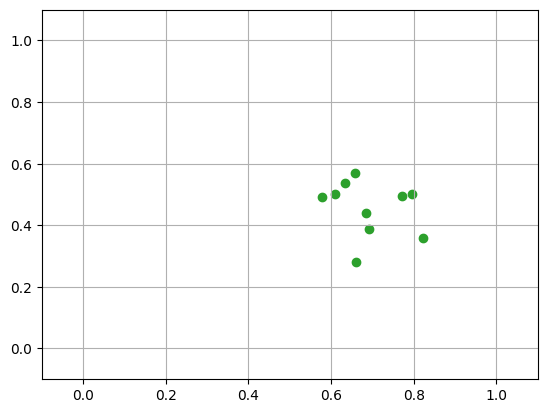
\includegraphics[width=\textwidth]{images/sim-search-knn}
            \caption*{\(\mathcal{K}\)}
        \end{subfigure}
    \hfill
        \begin{subfigure}{0.24\textwidth}
            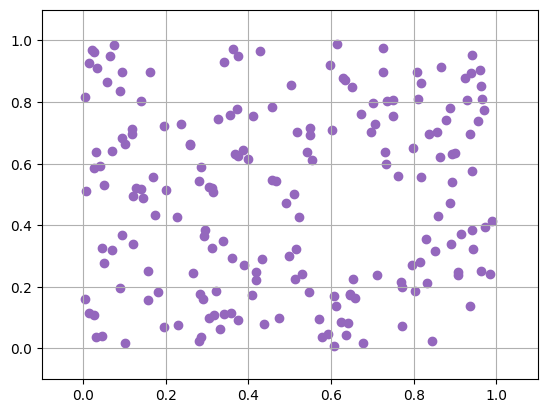
\includegraphics[width=\textwidth]{images/sim-search-Pminus}
            \caption*{\(\mathcal{P} \setminus \mathcal{K}\)}
        \end{subfigure}
    \end{figure}
    \hfill
\end{frame}

\subsection{ANNS Graphs}

\begin{frame}{Why graph?}
    \begin{itemize}
        \item Big, high-dimensional data sets
        \item Exact solutions are expensive
        \item \{Tree, Hash\}-based solutions breaks down
            \begin{itemize}
                \item Curse of dimensionality
            \end{itemize}
        \item Graphs work better
    \end{itemize}
\end{frame}

\begin{frame}{Why remove?}
    \begin{itemize}
        \item Data becomes stale
        \item Existing algorithms don't do removal
        \item Challenges with removals:
            \begin{itemize}
                \item Disconnection
                \item Quality/Performance deprecation
            \end{itemize}
    \end{itemize}
\end{frame}

\begin{frame}
    \centering
    \textbf{Goal:} Design a data structure that supports efficient vertex removal.
\end{frame}
